\section{The Chain Index}\label{sec:index}
% 2026-09-21 house shape and cadence pass: overview + Figure 2; each block with its property, theorem, proof, example on
% Figures 1 and 2; the values block holds the certified tail; the size block closes with the accounting.

This section answers the second difficulty of Section~\ref{sec:intro}: how to return any community of any size as a few ranges of labels.
%
The index has three parts: the vertex-to-chain map, one record per chain, and for every size one tree over the chains with an array of runs (Section~\ref{sec:runs}).
%
We call the tree of a size with its runs the \textit{layer} of that size.
%
Figure~\ref{fig:layout} draws the three parts for the running example, and traces one community query through them.
% 2026-09-22 filler pass: the roadmap of the subsections removed.

\begin{figure*}[t]
\centering
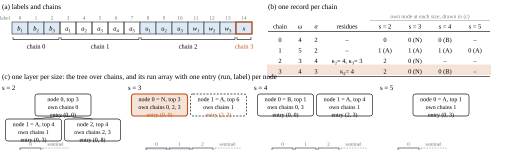
\includegraphics[width=\textwidth]{figures/fig_index.pdf}
\caption{\chainidx for Figure~\ref{fig:example}: (a) the labels and the four chains, (b) the record of every chain, (c) the layer of every size, and the community query of $x$ at $(3,2)$ traced through them (Example~\ref{ex:query}).}\label{fig:layout}
\end{figure*}

\subsection{Aligned labels}\label{sec:labels}
% 2026-09-22 compaction: the map in five sentences, the example in three (labels [0,3), [3,8), [8,14), [14,15) from make_concept.py).
Chains partition $V$ (Section~\ref{sec:chains}), so the vertices can be relabelled so that every chain is one interval of labels: the chains are numbered $0$ to $C-1$ in the order of Section~\ref{sec:order}, and the interval of a chain runs from its first label to the first label of the next chain.
%
The chain of $v$, written $\mathrm{chain}(v)$, is the number of chain starts, the first labels of the chains, at or before the label of $v$, minus one.
%
This is a rank query over the $n$ labels with the $C$ chain starts marked, and it takes constant time with $n+o(n)$ bits~\cite{Jacobson1989}.
%
The map stores those bits and the first label of every chain.
%
A community is a union of chains (Lemma~\ref{lem:union}) and so a list of label ranges.
%
If the graph is kept under its original ids, the index also stores the permutation from ids to labels, $n$ labels.
\begin{example}\label{ex:labels}
Figure~\ref{fig:layout} numbers the four chains of Example~\ref{ex:chains} in the order of Section~\ref{sec:order}: chain $0$ is $\{b_1,b_2,b_3\}$ with the labels $[0,3)$, chain $1$ is $\{a_1,\dots,a_5\}$ with $[3,8)$, chain $2$ is $\{u_1,\dots,w_3\}$ with $[8,14)$, and chain $3$ is $\{x\}$ with $[14,15)$.
%
The chain starts are the labels $0$, $3$, $8$ and $14$.
%
The vertex $u_1$ has label $8$, three starts lie at or before it, and its chain is $3-1=2$.
\end{example}

\subsection{Chain order}\label{sec:order}
The number of ranges an answer needs depends on the order of the chains.
%
The vertices of a chain $c$ share their own node at every size, written $\own{s}{c}$.
%
Fix any preorder numbering $\mathrm{pre}_s$ of each forest $\Tree{s}$, give chain $c$ the key $(\mathrm{pre}_2(\own{2}{c}),\mathrm{pre}_3(\own{3}{c}),\dots)$, the preorder positions of its own nodes size by size, and rank the chains in lexicographic key order.
%
The chain of the vertices in no edge has an empty key and is placed last.
\begin{theorem}[single ranges at size 2]\label{thm:onerange}
Under the lexicographic order, the labels of every $\Nuc{2}{k}$ form one interval.
\end{theorem}
\begin{proof}
An $\Nuc{2}{k}$ is the vertex set of the subtree of $\Tree{2}$ rooted at some node $X$.
%
A chain $c$ lies in it if and only if its own node $\own{2}{c}$, the smallest node containing $c$, is in that subtree.
%
The preorder numbers of a subtree form an interval, and the chains whose first key component lies in an interval are contiguous in lexicographic order.
%
Contiguous ranks are contiguous labels.
\end{proof}
\begin{example}\label{ex:order}
% trace 2026-09-22 (make_concept.py): keys (0,0,0), (1,1,1,0), (2,0), (2,0,0) with pre_2: root=0, A=1, {x,u,w}=2; pre_3: N=0, A=1; pre_4: B=0, A=1.
In Figure~\ref{fig:layout}(c), at size $2$ the root is node $0$, $A$ is node $1$ and $\{x,u_1,\dots,w_3\}$ is node $2$, so the keys are $(0,0,0)$ for $\{b_1,b_2,b_3\}$, $(1,1,1,0)$ for $\{a_1,\dots,a_5\}$, $(2,0)$ for $\{u_1,\dots,w_3\}$ and $(2,0,0)$ for $\{x\}$, the own-node columns of Figure~\ref{fig:layout}(b).
%
The shorter key ranks first, which gives the chains $0$ to $3$ and their labels.
%
The $(2,4)$-core $\{x,u_1,\dots,w_3\}$ is the interval $[8,15)$, and the $(2,3)$-core is $[0,15)$.
\end{example}
\begin{corollary}\label{cor:kcore}
The size-$2$ layer of the index is an index for connected $k$-core communities in which every community is one label range.
\end{corollary}
% 2026-09-22 filler pass: the comparison with k-core indexes after the corollary moved to Section 9 (it was already there).

\subsection{Run arrays and entry points}\label{sec:runs}
% 2026-09-22 prose pass: "active" glossed; the traversal rule in two sentences; the s=2 claim carries its reason; lo/hi defined.
% 2026-09-22 compaction: the array, the traversal rule, runs and entries in seven sentences.
A chain is \textit{active} at size $s$ when $s$ is at most its clique number.
%
The \textit{depth-first array} of size $s$ lists the active chains in a depth-first traversal of $\Tree{s}$ that, at each node, lists the chains whose own node it is and the subtrees of its children in increasing order of the smallest chain rank each contains, a chain counting as its own rank, and that orders the roots in the same way.
%
The chains of any subtree are then one contiguous segment of the array, starting with the chain of smallest rank in the subtree.
%
The order in which the traversal visits the nodes is a preorder of $\Tree{s}$, the \textit{traversal order}, in general different from $\mathrm{pre}_s$.
%
For $s=2$ the array is the rank order itself, since the first key component places the chains of a node before its subtrees and the subtrees in the order of $\mathrm{pre}_2$.
%
Two chains listed one after the other whose ranks differ by one own adjacent label intervals; maximal sequences of such chains are merged into \textit{runs}, numbered $0$ to $R-1$, and run $r$ covers the labels from $\mathrm{lo}(r)$ to $\mathrm{hi}(r)$, the latter excluded.
%
Every node $X$ stores one \textit{entry} $(r_X,v_X)$, the number of the run that holds the first label of the segment of $X$ and that label, and a sentinel entry $(R,\mathrm{hi}(R-1))$ follows the last node.
\begin{theorem}[retrieval]\label{thm:retrieval}
Let $Y$ be the node that follows the subtree of $X$ in the traversal order, or the sentinel if there is none.
%
If $r_X=r_Y$, the labels of the vertices of $X$ are the one range $[v_X,v_Y)$.
%
Otherwise they are the first range $[v_X,\mathrm{hi}(r_X))$, the whole runs $r_X+1,\dots,r_Y-1$, and the last range $[\mathrm{lo}(r_Y),v_Y)$.
%
When $Y$ is the sentinel there is no last range.
%
The number of nonempty ranges equals the number of runs that meet the segment, and at $s=2$ it is one.
\end{theorem}
\begin{proof}
The segment of $X$ in the depth-first array starts at the first chain of $X$ and ends before the first chain of $Y$, or at the end of the array when $Y$ is the sentinel.
%
Runs are maximal over the whole array, so inside the segment a run can be cut only at the two ends of the segment.
%
The run $r_X$ contributes its labels from $v_X$ on, the runs strictly between $r_X$ and $r_Y$ are whole, and the run $r_Y$ contributes its labels before $v_Y$, an empty range when the segment ends at a run boundary.
%
If $Y$ is the sentinel, the segment ends with run $R-1$, which is whole.
%
Each run that meets the segment gives one range, and at $s=2$ the whole array is one run, since it is the rank order.
\end{proof}
\begin{example}\label{ex:runs}
Consider the layer $s=3$ in Figure~\ref{fig:layout}.
%
The traversal lists $N$ before $A$, since $N$ holds chain $0$, and the chains of $N$ in rank order, so the depth-first array is chain $0$, chain $2$, chain $3$, chain $1$.
%
Chains $2$ and $3$ have consecutive ranks and merge into one run, and the array is stored as the three runs $[0,3)$, $[8,15)$, $[3,8)$ with the entries $N\to(0,0)$, $A\to(2,3)$ and the sentinel $(3,8)$.
%
The community of $x$ at $(3,2)$, traced in Figure~\ref{fig:layout}, is $N$, followed by $A$ with $r_N=0\ne r_A=2$: the first range $[0,3)$, the whole run $[8,15)$ and the empty last range $[\mathrm{lo}(2),3)=[3,3)$, two ranges for ten vertices.
%
The community $A$ at $(3,6)$ is followed by the sentinel, $r_A=2\ne3$, and is the first range $[3,\mathrm{hi}(2))=[3,8)$ alone.
\end{example}

\subsection{Values}\label{sec:values}
% 2026-09-21 the certified tail moved here from the former hierarchy section (house order: the theorem where it is used).
Core values are constant on a chain (Theorem~\ref{thm:chains}), and so is the clique number, the last size with a nonzero value.
%
% 2026-09-22 compaction: the floor and the announcement in three sentences.
Inside its largest clique alone, a vertex lies in $\binomc{\omg{v}-1}{s-1}$ $s$-cliques, so its value at size $s$ cannot fall below this number, its \textit{floor} at size $s$.
%
The next theorem says that once the value reaches the floor at some size, it stays on the floor at every larger size, so most values need not be stored.
%
Its proof uses the Kruskal--Katona theorem in Lov\'asz's form \cite{kruskal1963,katona1968,lovasz1979}, with the binomial coefficient $\binomc{t}{s}=t(t-1)\cdots(t-s+1)/s!$ extended to real $t$; for $t\ge s-1$ both $\binomc{t}{s}$ and $\binomc{t}{s-1}$ increase strictly with $t$.
\begin{lemma}[Kruskal--Katona]\label{lem:kk}
For $m\ge1$ let $t\ge s$ be the real number with $\binomc{t}{s}=m$.
%
Any $m$ or more distinct $s$-element sets have at least $g_s(m)=\binomc{t}{s-1}$ distinct $(s-1)$-element subsets.
\end{lemma}
\begin{theorem}[floor and certified tail]\label{thm:tail}
Let $2\le s\le\omg{v}$.
\begin{enumerate}[label=(\alph*),leftmargin=*,nosep]
\item $\core{s}{v}\ge\binomc{\omg{v}-1}{s-1}$.
\item If $\core{s}{v}=\binomc{\omg{v}-1}{s-1}$ and $s<\omg{v}$, then $\core{s+1}{v}=\binomc{\omg{v}-1}{s}$.
\end{enumerate}
\end{theorem}
\begin{proof}
(a) A largest clique $L$ containing $v$ has $\omg{v}$ vertices.
%
Every vertex of $L$ lies in $\binomc{\omg{v}-1}{s-1}$ $s$-cliques of $L$, and $L$ is connected through them, so $L$ has the two properties at the level of the floor and lies inside a core of size $s$ at that level.

(b) Let $K$ be the $\Nuc{s+1}{\core{s+1}{v}}$ containing $v$, and take any vertex $u$ of $K$.
%
It lies in at least $\core{s+1}{v}$ cliques of $s+1$ vertices inside $K$, and removing $u$ from them leaves as many distinct $s$-element sets of neighbours of $u$ in $K$.
%
By Lemma~\ref{lem:kk} these sets have at least $g_s(\core{s+1}{v})$ distinct $(s-1)$-element subsets, and each of them forms with $u$ an $s$-clique of $K$.
%
Every vertex of $K$ hence lies in at least $g_s(\core{s+1}{v})$ $s$-cliques of $K$.
%
$K$ is connected through these $s$-cliques, because two $(s+1)$-cliques that share a vertex contain $s$-cliques that share it, and hence $\core{s}{v}\ge g_s(\core{s+1}{v})$.
%
If $\core{s+1}{v}>\binomc{\omg{v}-1}{s}$, then the $t$ with $\binomc{t}{s}=\core{s+1}{v}$ exceeds $\omg{v}-1\ge s$, so $\core{s}{v}\ge\binomc{t}{s-1}>\binomc{\omg{v}-1}{s-1}$, contradicting the assumption of (b).
%
Since $\core{s+1}{v}\ge\binomc{\omg{v}-1}{s}$ by (a), equality holds.
\end{proof}
We write $\sig{v}$, the \textit{certification point}, for the smallest size at which the value equals the floor, and we set $\sig{v}=\omg{v}+1$ when no size does.
%
For $s\ge\sig{v}$ the value is $\binomc{\omg{v}-1}{s-1}$, by (b) applied size after size, and is not stored.
%
The values for $2\le s<\sig{v}$ are the \textit{residue} of $v$.
\begin{example}\label{ex:tail}
% trace 2026-09-22 (make_concept.py): sigma = 2 on A and B's b_i, 3 on x, 4 = omega+1 on u,w; residues: chain 2 (4, 3), chain 3 (4).
In Figure~\ref{fig:example}, the vertices of $A$ have clique number $5$ and $\core{2}{a_i}=4=\binom{4}{1}$, so $\sig{a_i}=2$ and no value of $A$ is stored: $\core{3}{a_i}=\binom{4}{2}=6$, $\core{4}{a_i}=\binom{4}{3}=4$ and $\core{5}{a_i}=\binom{4}{4}=1$ are read from the floor.
%
The vertices $b_i$ have clique number $4$ and $\core{2}{b_i}=3=\binom{3}{1}$, so $\sig{b_i}=2$ as well.
%
The vertex $x$ has $\core{2}{x}=4>\binom{3}{1}$ and $\core{3}{x}=3=\binom{3}{2}$, so $\sig{x}=3$ and its residue is the single value $\core{2}{x}=4$.
%
The six vertices $u_1,\dots,w_3$ have clique number $3$, $\core{2}{u_i}=4>\binom{2}{1}$ and $\core{3}{u_i}=3>\binom{2}{2}$, so no size reaches the floor, $\sig{u_i}=4=\omega+1$, and both values are residues.
%
Stored per chain, the whole graph keeps three values, the residues column of Figure~\ref{fig:layout}(b).
\end{example}
The record of a chain holds its clique number $\omega$, its certification point $\sigma$, its residues, and its trajectory (Definition~\ref{def:chain}), from which the community query starts.
%
Every value at or past $\sigma$ is the binomial coefficient of Theorem~\ref{thm:tail}, and for $s>\omega$ it is $0$.
%
The residues and the tops of one size are integers at most the largest core value of that size, and the index stores them at that length.

\subsection{Size}\label{sec:size}
Recall that $C$ is the number of chains, and let a word hold one label, one node or one value.
%
The map takes $n+o(n)$ bits and $C$ words for the first labels.
%
The chain records take $2C$ words for $\omega$ and $\sigma$, one word per (chain, size) pair for the trajectories, and one word per residue.
%
The layers take a constant number of words per canonical node, a parent, a top, a subtree size (which locates the node after the subtree, Section~\ref{sec:queries}) and an entry, and two labels per run.
%
\strees takes one word per (vertex, size) pair for its per-size arrays, as many words for its own-node pointers, a value for each of these pairs, and a constant number of words per canonical node.
%
Per node the layers of \chainidx cost more, an entry and a subtree size in addition.
%
The saving is in the stored units, $\sum_v(\omg{v}-1)$ (vertex, size) pairs against $\sum_c(\omega(c)-1)$ (chain, size) pairs, and in the values, the residues against a value per pair.
%
On the running example the index stores $3$ values, $8$ words for $\omega$ and $\sigma$ and $12$ trajectory words, while \strees stores $44$ values and $44$ own-node pointers, one per (vertex, size) pair.
% trace 2026-09-21: active pairs = a_i: sizes 2..5 = 4 each, 20; b_i: sizes 2..4 = 3 each, 9; x: 3; u_i,w_i: sizes 2,3 = 2 each, 12; total 44.
